\documentclass[tikz, 11pt]{standalone}

\usepackage{tikz}
\usetikzlibrary{shapes.geometric, arrows.meta, calc, decorations.pathmorphing}

% Clock paramters
\newcommand{\clockRadius}{10mm}
\newcommand{\hourHand}{5mm}
\newcommand{\minuteHand}{6mm}
\newcommand{\tickLength}{2mm}
\newcommand{\clockStartAngle}{210}
\newcommand{\clockEndAngle}{-15}
\newcommand{\plugRadius}{2mm}
\newcommand{\plugLeg}{1.5mm}
\newcommand{\arrow}{{Latex[length=2mm, width=5mm]}}
\newcommand{\lineWidth}{3pt}
\newcommand{\fontSize}{16}

% Bar paramters
\newcommand{\barWidth}{5mm}
\newcommand{\barHeight}{8mm}
\newcommand{\barInc}{1.5mm}
\newcommand{\linePad}{0.5mm}

% Colors
\definecolor{lineColor}{RGB}{0, 0, 0}
\definecolor{barOrange}{RGB}{234,120,72}
\definecolor{barGray}{RGB}{170,182,186}
\definecolor{barGreen}{RGB}{87,175,70}

% Styles
\tikzstyle{panel}=[draw=none, inner sep=0, outer sep=0]
\tikzstyle{bar}=[panel, fill=barGray, minimum width=\barWidth, minimum height=\barHeight, rounded corners=1mm, draw=none, line width=\lineWidth]
\tikzstyle{line}=[draw=lineColor, line width=\lineWidth, cap=round]
\tikzstyle{lines}=[line, rounded corners=1mm]
\tikzstyle{arrow}=[line, -\arrow]
\tikzstyle{textNode}=[draw=none, inner sep=2mm]
\tikzstyle{textLabel}=[draw=none, inner sep=0, outer sep=0, text height=7pt, text depth=2pt]

\begin{document}

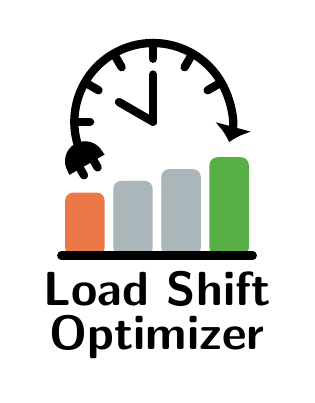
\begin{tikzpicture}[]

% Frame
%\node[panel, draw=red, minimum width=4.5cm, minimum height=4.5cm, yshift=-10mm] (frame) at (0,0) {};

% Useful coordinates
\coordinate (clockStart) at (\clockStartAngle:\clockRadius);
\coordinate (clockEnd) at (\clockEndAngle:\clockRadius);

% Clock circle
\draw[arrow] 
  (clockStart) arc 
  (\clockStartAngle:\clockEndAngle:\clockRadius); 
% Hands
\draw[line] (0,0) -- (150:\hourHand);
\draw[line] (0,0) -- (90:\minuteHand);
% Ticks
\foreach \a in {30,60,...,180} {
  \draw[line] (\a:\clockRadius-\tickLength) --(\a:\clockRadius);
  }
% Plug
\begin{scope}[rotate=\clockStartAngle-180]
  \draw[line, fill=black] ($(clockStart)+(-\plugRadius, 0)$)
        arc[start angle=180, end angle=0, radius=\plugRadius] -- cycle;
  \draw[line] ($(clockStart)+(-0.5*\plugRadius, 0)$) --++ (0, -\plugLeg);
  \draw[line] ($(clockStart)+(0.5*\plugRadius, 0)$) --++ (0, -\plugLeg);
\end{scope}

% Bars
\node[bar, anchor=north, fill=barOrange, yshift=-4mm] (barLeft) at (clockStart) {};
\node[bar, anchor=south, fill=barGreen, minimum height=\barHeight+3*\barInc] (barRight) at (clockEnd|-barLeft.south) {};
\node[bar, anchor=south, minimum height=\barHeight+1*\barInc] at ($(barLeft.south)!1/3!(barRight.south)$) {};
\node[bar, anchor=south, minimum height=\barHeight+2*\barInc] at ($(barLeft.south)!2/3!(barRight.south)$) {};
\draw[line] ([xshift=-\linePad]barLeft.south west) -- ([xshift=\linePad]barRight.south east);

% Text label
\node[
  textNode, 
  align=center, 
  text=lineColor, 
  font=\sffamily\bfseries\fontsize{\fontSize}{\fontSize}\selectfont, 
  anchor=north] 
  at ($(barLeft.south)!1/2!(barRight.south)$) {Load Shift \\Optimizer};

\end{tikzpicture}
\end{document}